\documentclass[a4paper,twoside,twocolumn]{article}
\pdfoutput=1

\newif\iftr % \trtrue if for Tech Report
\trtrue     % \trfalse if not for Tech Report
%\newif\ifnony % \nonytrue if nonymised (ie nameful)
%\nonyfalse     % \nonyfalse if anonymised

% Test whether compiler is PDFLaTeX
\usepackage{ifpdf}  % Avoid \newif\ifpdf which clashes with same command
                    % in ifpdf package used by packages like hyperref
\ifpdf
    \usepackage[pdftex]{graphicx}
    \usepackage[colorlinks,linkcolor=blue,citecolor=blue,urlcolor=blue]{hyperref}
    \pdfcompresslevel=9 % Maximum compression
    \DeclareGraphicsExtensions{.pdf}
    % \usepackage[pdftex]{thumbpdf}      % thumbnails for pdflatex
    \pdfadjustspacing=1                % force LaTeX-like character spacing
\else
    \usepackage{graphicx}
    \usepackage[hypertex]{hyperref}  % supports hypertext in PDF but no Acrobat features e.g. bookmarks
\fi
% Common settings for hyperref are made in hyperref.cfg

% Load packages that require graphicx to have been loaded.
\usepackage{todonotes} % clashes with pdftex option below
%\usepackage[disable]{todonotes} % Suppresses todo notes
\newcommand{\bob}[1]{\todo[color=olive!40,inline]{Bob: #1}}
\newcommand{\vidhi}[1]{\todo[color=orange!40,inline]{Vidhi: #1}}

% Load supported packages
\usepackage{
url       %
,fancyhdr % Fancy Headers
,lastpage % Creates marker with key LastPage, for pxxx of yyy to refer to.
,enumerate % More bullet styles
,amsmath  % AMS maths
,amsfonts % AMS fonts
,amssymb  % AMS symbols
,multirow % multi-row cells in tables
,xcolor   % color definitions
,colortbl % coloured columns
%,moreverb % additional verbatim miscellany
%,amsthm   % AMS theorems defines proof environment
%,calc     % For calculations in length commands
%,newtheorems % Load after hyperref: see below
, enumitem % finer control of lists, e.g. \begin{itemize}[nosep] ... removes spacing
}
%\usepackage[force,almostfull]{textcomp} % Additional symbols, including generic currency
\usepackage[hang]{footmisc} % Hanging indent for footnotes
\setlength\footnotemargin{10pt}
\usepackage{balance}

% Load my personal packages
\usepackage[noindent, arraystretch, fullpage]{setlengths} % [noindent, arraystretch, {fullpage|tightpage|inchrndtext}]{setlengths}
\usepackage{
own         % Defines \newboolean{twocol}
}

% Load my personal packages
%\usepackage{
%newtheorems, % Defines theorem, definition, hypothesis, lemma \& assumption environments
%             % Note: \newtheorem must be used after \usepackage{hyperref} to ensure \theH<counter> is cross-referenced as well as \the<counter>
%}
\usepackage{amsthm}
\newtheorem{assumption}{Assumption}
\newtheorem{requirement}{Requirement}
\newtheorem*{test*}{Test}
\usepackage{xfrac}

\definecolor{Grey}{gray}{0.85}
\definecolor{good}{rgb}{0.85,1,0.85}
\definecolor{bad}{rgb}{1,0.85,0.85}
\newcolumntype{G}{>{\columncolor{Grey}}c}
\newcolumntype{g}{>{\columncolor{good}}c}
\newcolumntype{b}{>{\columncolor{bad}}c}


\graphicspath{{images/}}

% Preamble metadata---------------------------------------------------
\newcommand*{\metaauthori}{Bob Briscoe}
\newcommand*{\metashorttitle}{ECN Tunnelling Test}
\newcommand*{\metatitle}{A Test for IP-ECN Propagation by a Remote Tunnel Endpoint}
\newcommand*{\metano}{TR-BB-2023-003}
\newcommand*{\metakeywords}{Data Communication, Networks, Internet, Control, Active Queue Management, AQM, Pacing,  Medium Access Delay, MAC delay, Congestion Control, Quality of Service, Policing, Burstiness, Performance, Algorithm, Standards}
\newcommand*{\metahomepage}{\(<\)\href{http://bobbriscoe.net/}{http://bobbriscoe.net/}\(>\)}
\newcommand*{\metamaili}{\href{mailto:research@bobbriscoe.net}{research@bobbriscoe.net}}
\newcommand*{\metaaddress}{}
\newcommand*{\metatel}{Tel. +44 7718 902848}
\newcommand*{\metaversion}{01}
\newcommand*{\metadate}{28 Nov 2023}

\hypersetup{                       % Set PDF document attributes
%     pdfauthor = {\metaauthori and \metaauthorii
     pdfauthor = {\metaauthori
     },
     pdftitle = {\metashorttitle},
     pdfsubject = {},
     pdfkeywords = {\metakeywords}
}%

% Set document metadata
\title{\metatitle}%
\author{\metaauthori%
\thanks{\metamaili, %
\metaaddress}%
\ %
%\and \metaauthorii%
%\thanks{\metamailii}%
}
\date{\metadate}%

% Running headers and footers
\pagestyle{fancy}%
\fancyhf{}%
\fancyhead[LO,RE]{\metashorttitle}%
\fancyhead[LE,RO]{\metano}%
\fancyfoot[LO,RE]{\scriptsize{\copyright~bobbriscoe.net Ltd, 2023}}%
%\fancyfoot[LO,RE]{}%
\cfoot{\footnotesize{\scriptsize{Version~\metaversion}}}%
\fancyfoot[RO,LE]{\scriptsize{\thepage~of~\pageref{LastPage}}}%

\fancypagestyle{first}{%
\fancyhead[LO,RE]{}%
\fancyhead[LE,RO]{}%
%\fancyhead[C]{\Large Draft: Limited Review Distribution only}%
\fancyhead[C]{}%
\renewcommand{\headrulewidth}{0pt}%
}%

% Typesetting control
\pretolerance = 150%
%\tolerance = 250%
\tolerance = 5000%
\emergencystretch = 0 em%
% Typesetting overfull/underfull message control
%\hbadness = 150%
\hbadness = 4999%
\hfuzz = 0 pt%

% Set amsmath equation numbering to be relative to containing section
%\numberwithin{equation}{section}
%\newcounter{req}

% Set Sectioning style
%\setcounter{secnumdepth}{3}
%\renewcommand{\baselinestretch}{1.2}
%\renewcommand{\bibname}{References}

% ----------------------------------------------------------------
\begin{document}
\bibliographystyle{alpha}%

% ----------------------------------------------------------------

\maketitle%
%\bob{ToDo: Add authors or acknowledge others}
\thispagestyle{first}

% ----------------------------------------------------------------
\begin{abstract}
{\small\noindent%
% !TeX root = ecn-encap-test_tr
% ================================================================

This memo defines a brief set of tests to determine the decapsulation behaviour
of an unknown remote tunnel endpoint with respect to the Explicit Congestion
Notification (ECN) field in the Internet Protocol (IP) header. The tests could
be automated to be used by a tunnel ingress to determine whether the egress that
it is paired with will propagate ECN correctly.


}      % Abstract
\end{abstract}
% !TeX root = ecn-encap-test_tr
% ================================================================
\section{Introduction}\label{ecn-encap-test_Intr}

This memo defines a brief set of tests to determine the decapsulation behaviour of an unknown remote tunnel endpoint, with respect to the ECN field in the IP header. It provides a table that says whether each possible detected behaviour will propagate ECN correctly.

Test prerequisites are given in \S\,\ref{ecn-encap-test_Prereq}, the main hurdle being the ability to overwrite the ECN field in the outer header at some point along the span of a tunnel. This makes it hard to test `bump in the wire' tunnels. To overcome this hurdle, a convenient arrangement would be to set up the ingress of the tunnel under test on a host under the control of the tester. 

The tests could be automated to be used by a tunnel ingress to determine whether the egress it is paired with will propagate ECN correctly. Without such a test, a tunnel ingress is required to zero the outer ECN field if it does not know whether the egress it is paired with will propagate ECN correctly~\cite{Briscoe16b:ecn-tunnel-scope_ID}. 

In scenarios where there is no control protocol for a tunnel ingress to discover the ECN capability of the egress, such a test could widen ECN coverage to tunnelled paths where it is currently absent.

\subsection{Terminology}\label{ecn-encap-test_Term}

\begin{description}
	\item[Encap:] the encapsulation function at the ingress tunnel endpoint;
	\item[Decap:] The decapsulation function at the egress tunnel endpoint;
\end{description}

The following terms will be used for the IP header at different locations on the path relative to the tunnel, considering only the direction from application client to application server:
\begin{description}
	\item[Initial:] the header arriving at the tunnel ingress;
	\item[Inner:] the header that is encapsulated between the tunnel ingress and egress;
	\item[Outer:] the header that encapsulates the inner between the tunnel ingress and egress;
	\item[Onward:] the header leaving the tunnel egress.
\end{description}
      % Intro
% !TeX root = ecn-encap-test_tr
% ================================================================
\section{The Tests}\label{ecn-encap-test_Test}

% ----------------------------------------------------------------
\subsection{Test Prerequisites}\label{ecn-encap-test_Prereq}

\begin{itemize}[nosep]
	\item A working tunnel, e.g.\ a VPN;
	\item Access to one of the devices along the path of the tunnel, where the ECN field of the outer IP header can be altered\footnote{Ideally so it can be altered arbitrarily, but just being able to set congestion experiences (CE, i.e. 0b11) would support all the tests except one, which is a less important one anyway.};
	\item A remote application server, e.g.\ a web server (preferably a variety of different servers) that supports Accurate ECN feedback over either TCP~\cite{Briscoe14d:accecn_ID} or QUIC~\cite{Iyengar21:QUIC}.
	\item A local application client (e.g.\ a web browser), optionally with the ability to configure whether it sends ECN-capable packets (prior to tunnelling), and if so whether it sets ECT(0) or ECT(1). 
\end{itemize}
% ----------------------------------------------------------------
\subsection{Test Setup}\label{ecn-encap-test_Setup}

Set up the tunnel as normal (procedure will depend on which type of tunnel).

\paragraph{If using TCP} configure the client TCP stack to use Accurate ECN (AccECN) feedback: 
\begin{description}[style=nextline, nosep]
	\item[Linux:] \texttt{\$ sysctl -w net.ipv4.tcp\_ecn=3}
	\item[MacOS:] \texttt{\$ sysctl -w net.inet.tcp.accurate\_ecn=1}
\end{description}

\paragraph{If using QUIC} make sure your QUIC implementation supports accurate ECN feedback (at the time of writing, some still don't comply with the spec~\cite{Iyengar21:QUIC}).

Make sure your application traffic is being routed via the tunnel.

% ----------------------------------------------------------------
\subsection{Control Test}\label{ecn-encap-test_Control}

The aim of this control test is to send packets with each of the four ECN codepoints from the application client, then check that feedback from the application server reflects the same codepoint. 

Also it will be necessary to check that the tunnel ingress is copying each ECN codepoint to the outer. If it's not, in order to test the remote tunnel endpoint, it will be necessary to overwrite the outer with a copy of the Initial ECN codepoint (using a similar approach to that for the main tests in \S\,\ref{ecn-encap-test_Main}). 

\paragraph{Details:} The Initial IP-ECN field can either be controlled by configuring the client stack, or by overwriting the field in the packet before it enters the tunnel. Given all codepoints cannot be set by configuration on all packets, only the overwrite approach will be described here. One example technique is to use the \texttt{tc} (traffic control) command to add a filter that applies an action to packets matching the filter. The Linux \texttt{tc} command is used for the example here, but  \texttt{tc} is also available for MacOS.

\begin{verbatim}
$ tc filter add \
     dev DEV ingress flower MATCH_LIST \
     action pedit ex munge \
     ip dsfield set N retain 0x3
\end{verbatim}
where \texttt{N} would be respectively 0 to 3 to set the ECN field to Not-ECT, ECT(1), ECT(0) or CE. \texttt{DEV} might be \texttt{eth0} for example. And an example of a \texttt{MATCH\_LIST} might be \texttt{ip\_proto tcp dst\_port 80} (see the tc-flower manual page for details).

To check the Outer (outgoing) ECN, and the server's (incoming) feedback of the Onward ECN, Wireshark is recommended (version 4.0 onward supports AccECN in TCP). For this control test, check that the Initial is the same as the feedback of the Onward ECN, and that they are also the same as the Outer and the Inner.

The most specific feedback for testing purposes is given by TCP AccECN feedback in the SYN-ACK from the server in response to the initial TCP SYN packet from the client. The feedback is written with the `handshake encoding` into the three ECN flags (AE, CWR, ECE) in the main TCP header as in the following table (from Table 3 of \cite{Briscoe14d:accecn_ID}, which uses the TCP flags as newly defined in Figure 2 of the same draft):

%\begin{table}[h]
{\centering
\begin{tabular}{ccc}
	IP-ECN    & TCP-ECN  & Wireshark\\
	(outward) & (inward) &\\
	\hline%
	Not-ECT   & 0b010    & \texttt{.C.}\\
	ECT(1)    & 0b011    & \texttt{.CE}\\
	ECT(0)    & 0b100    & \texttt{A..}\\
	CE        & 0b110    & \texttt{AC.}\\
	\hline
\end{tabular}
\par}
%\end{table}

If your client sends data packets to the server once the TCP connection has been established, their feedback can be checked in AccECN TCP options that that server sends to the client. These give a count of how many bytes of each codepoint has been received by the server during the connection (counting from 1, not zero). However, they are not sent in response to every data packet (and they are optional). So further explanation will not be given, but if the reader wants to interpret this feedback, the definition of these TCP Options is in \S\,3.2.3 of \cite{Briscoe14d:accecn_ID}.

QUIC feedback can also be checked, but it has to be decrypted first. Apple gives instructions for how to allow Wireshark to decrypt QUIC for Cloudflare's quiche stack in order to check the ECN  feedback\footnote{\href{https://developer.apple.com/documentation/network/testing_and_debugging_l4s_in_your_app}{Testing and Debugging L4S in Your App}}, so that will not be repeated here. Then, any packet containing an ACK\_ECN frame can be viewed in Wireshark to read a count of the number of packets received by the server with each ECN codepoint: ECT(0), ECT(1) and ECN-CE.

\paragraph{Test robustness:} The test ought to be repeated a few times, and preferably conducted with a few different application servers (but over the same tunnel). This should help eliminate the possibility that:
\begin{itemize}[nosep]
	\item Active Queue Management (AQM) within the span of the tunnel is intermittently (and legitimately) setting the congestion experienced (CE) codepoint on the outer of some packets;
	\item A remote application server might have been chosen that provides incorrect ECN feedback due to an implementation bug.	
\end{itemize}

\begin{table*}
	{\centering
		\begin{tabular}{GGgggbb}
			\bf{Initial}&\bf{Outer}&\bf{RFC6040}&\bf{RFC4301}&\bf{RFC3168}&\bf{RFC2003}&\bf{mangled}\\
			&          &(unified)   &(IPsec)     &(original)  &(simple)    & \\
			\hline%
			Not-ECT     & CE       &dropped     &Not-ECT     & dropped    & Not-ECT    & \\
			ECT(1)      & CE       &CE          &CE          & CE         & ECT(1)     & \\
			ECT(0)      & CE       &CE          &CE          & CE         & ECT(0)     & \\
			ECT(0)      & ECT(1)   &ECT(1)      &ECT(0)      & ECT(0)     & ECT(0)     & \multirow{-4}{*}{other}\\
			\hline
		\end{tabular}
		\caption{Main Test: Possible Results and their Interpretation}\label{fig:Interpretation}
	}
\end{table*}

It should not be necessary to test both IPv4 \& IPv6 (and both combinations of the two), because the definition of ECN is the same in both, so ECN processing code should be common to both. However, a full test could include all four combinations of IPv4 \& IPv6.

% ----------------------------------------------------------------
\subsection{Main Test}\label{ecn-encap-test_Main}

To test for correct operation of the remote tunnel egress, it is only necessary to test the combinations in the first two (grey) columns of \autoref{fig:Interpretation} (in addition to the control test above).
%
%{\centering
%	\begin{tabular}{cc}
%		Initial    & Outer\\
%		\hline%
%		Not-ECT   & CE\\
%		ECT(1)    & CE\\
%		ECT(0)    & CE\\
%		ECT(0)    & ECT(1)\\
%		\hline
%	\end{tabular}
%\par}

For this test, the filter action will need to be applied after tunnel encapsulation. Then the outer will need to be overwritten with CE, for instance using the \texttt{tc} command as already outlined in \S\,\ref{ecn-encap-test_Control} with \(\mathtt{N}=\mathtt{3}\) (decimal), and in the case of the last row, with \(\mathtt{N}=\mathtt{1}\).

% ----------------------------------------------------------------
\subsection{Interpretation of Results}\label{ecn-encap-test_Interpretation}

If the results conform with any of the green columns in \autoref{fig:Interpretation}, the tunnel egress correctly propagates ECN-marking, because it either complies with the latest ECN tunnelling spec (RFC~6040~\cite{Briscoe07b:ECN-tunnel}) or with an earlier compatible spec updated by RFC~6040 (IPsec~\cite{IETF_RFC4301:IPSEC_architecture} or the original ECN spec~\cite{rfc3168}).

If, on the other hand, the results conform to one of the red columns, the tunnel egress does not propagate ECN correctly. For instance, the first red column shows the outcome of a `simple' tunnel, which just strips the outer on decapsulation (as used before ECN tunnelling was first specified in 2001). The final column `mangled' captures all other possible outcomes.
      % Body
%\input{ecn-encap-test_eval-data}      % Evaluation
%\input{ecn-encap-test_relwk-data}     % Related work
%\input{ecn-encap-test_tail-data}      % Tail pieces (discussion, conclusions, plans, acks)
% ----------------------------------------------------------------

%\onecolumn%
%\clearpage
\newpage
\addcontentsline{toc}{section}{References}

%\newpage
{%
%\footnotesize%
\scriptsize%
\bibliography{ecn-encap-test}}

% ----------------------------------------------------------------
\clearpage
%\twocolumn%
\appendix
% !TeX root = ecn-encap-test_tr
% ================================================================
\section{History of ECN propagation by tunnels}\label{ecn-encap-test_History}

\begin{figure}[h]
	\centering
	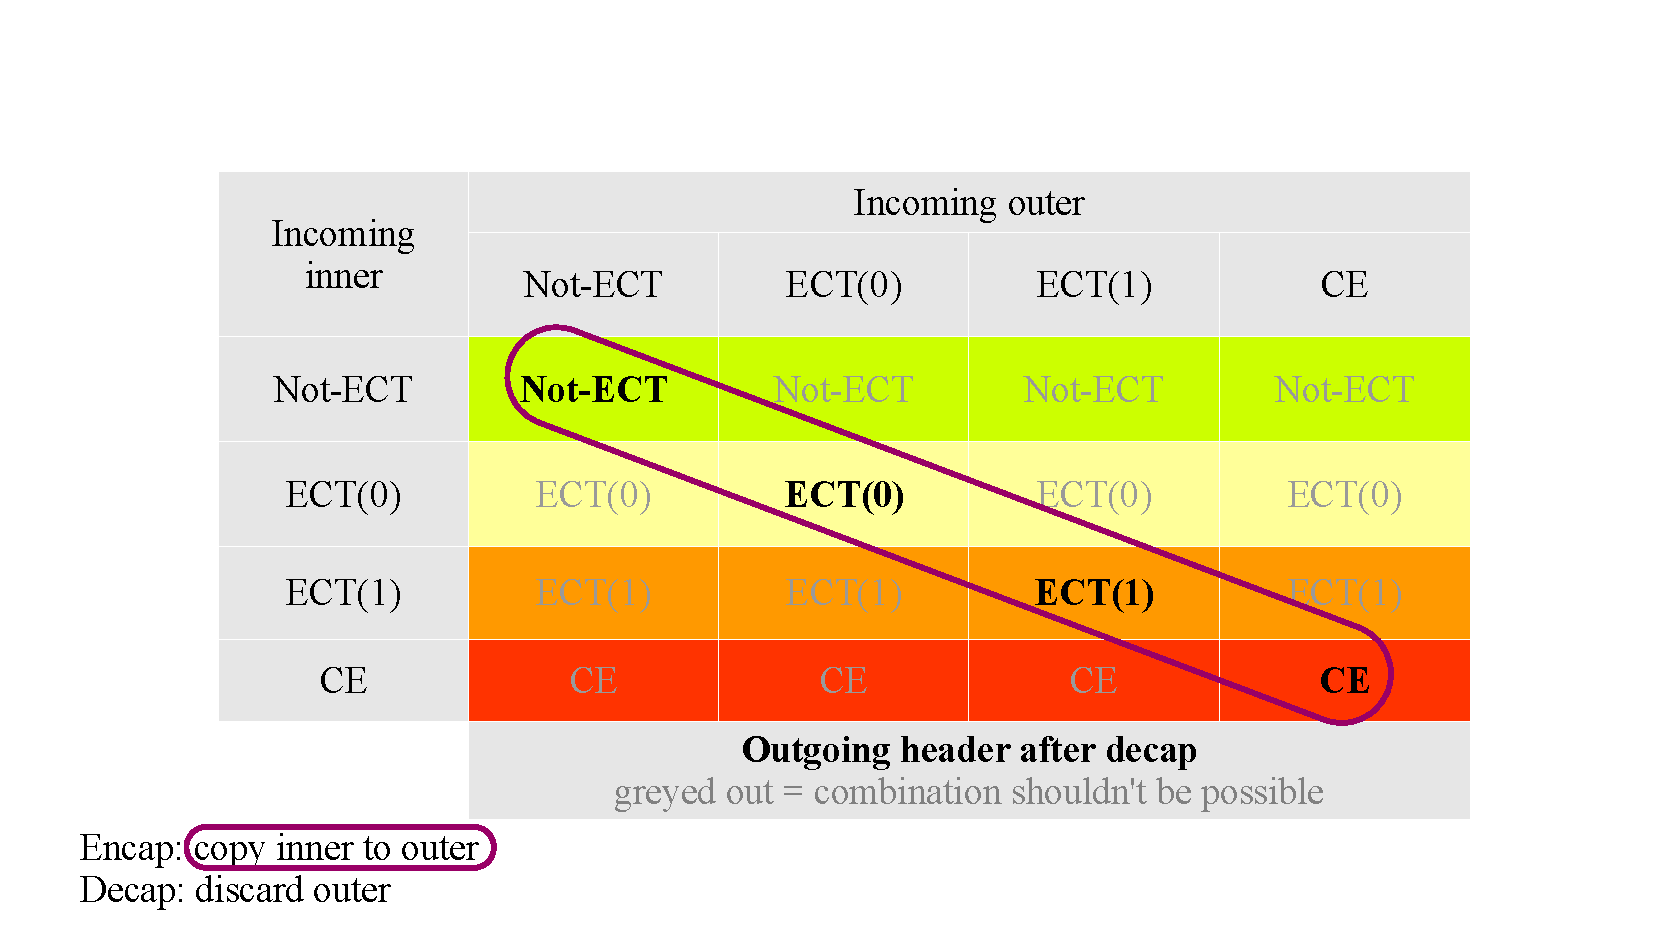
\includegraphics[width=\linewidth,clip]{ecn-tunnel-testing-bg-1}
	\caption{Simple (pre-ECN) tunnel, e.g.\ RFC2003}\label{fig:ecn-tunnel-testing-bg-1}
\end{figure}
\begin{figure}[h]
	\centering
	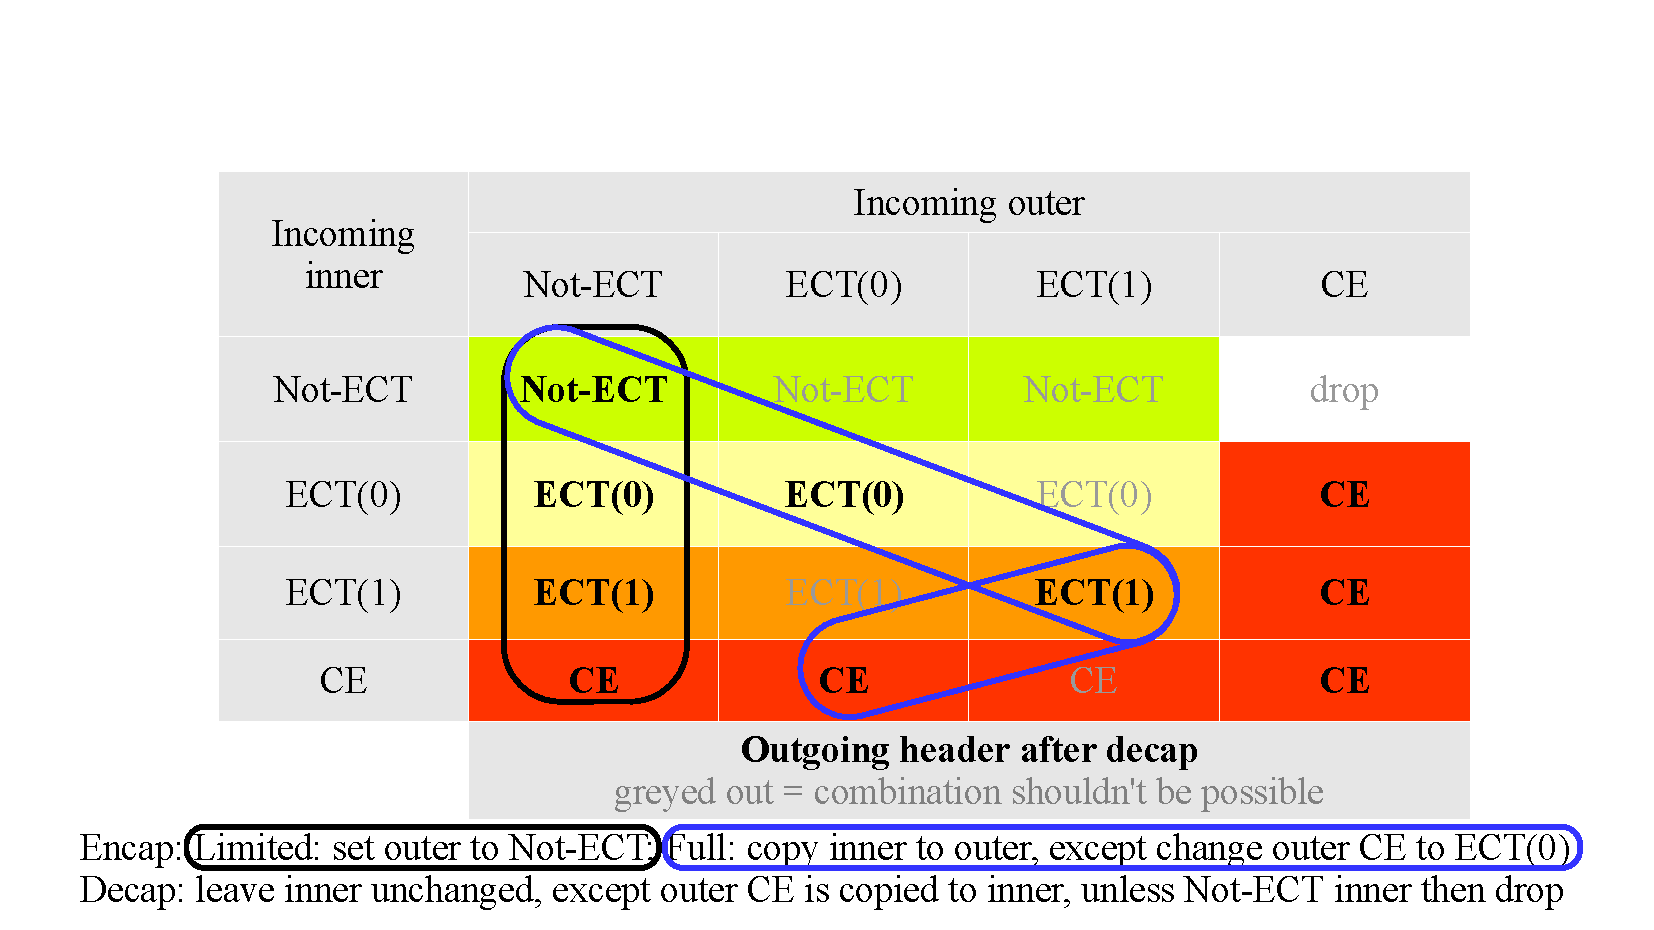
\includegraphics[width=\linewidth,clip]{ecn-tunnel-testing-bg-2}
	\caption{Original RFC~3168 ECN-tunnel~\cite{rfc3168}}\label{fig:ecn-tunnel-testing-bg-2}
\end{figure}

Figures \ref{fig:ecn-tunnel-testing-bg-1}--\ref{fig:ecn-tunnel-testing-bg-4} illustrate the evolution of ECN tunnelling, starting from pre-ECN days in \autoref{fig:ecn-tunnel-testing-bg-1}.

The table in each figure visualizes the outcome as each spec slightly altered the decapsulation rules. The rows represent the Inner and the columns represent the Outer header arriving at the tunnel egress. The text in each cell (and the associated background colour) gives the Onward (outgoing) header. 

The loops group together the combinations of Inner and Outer that would be expected, given the behaviour of an encapsulator that complies with the same spec as the decapsulator. Where the spec allows two encap options, different coloured loops are shown for each.

\newpage
\begin{figure}[h]
	\centering
	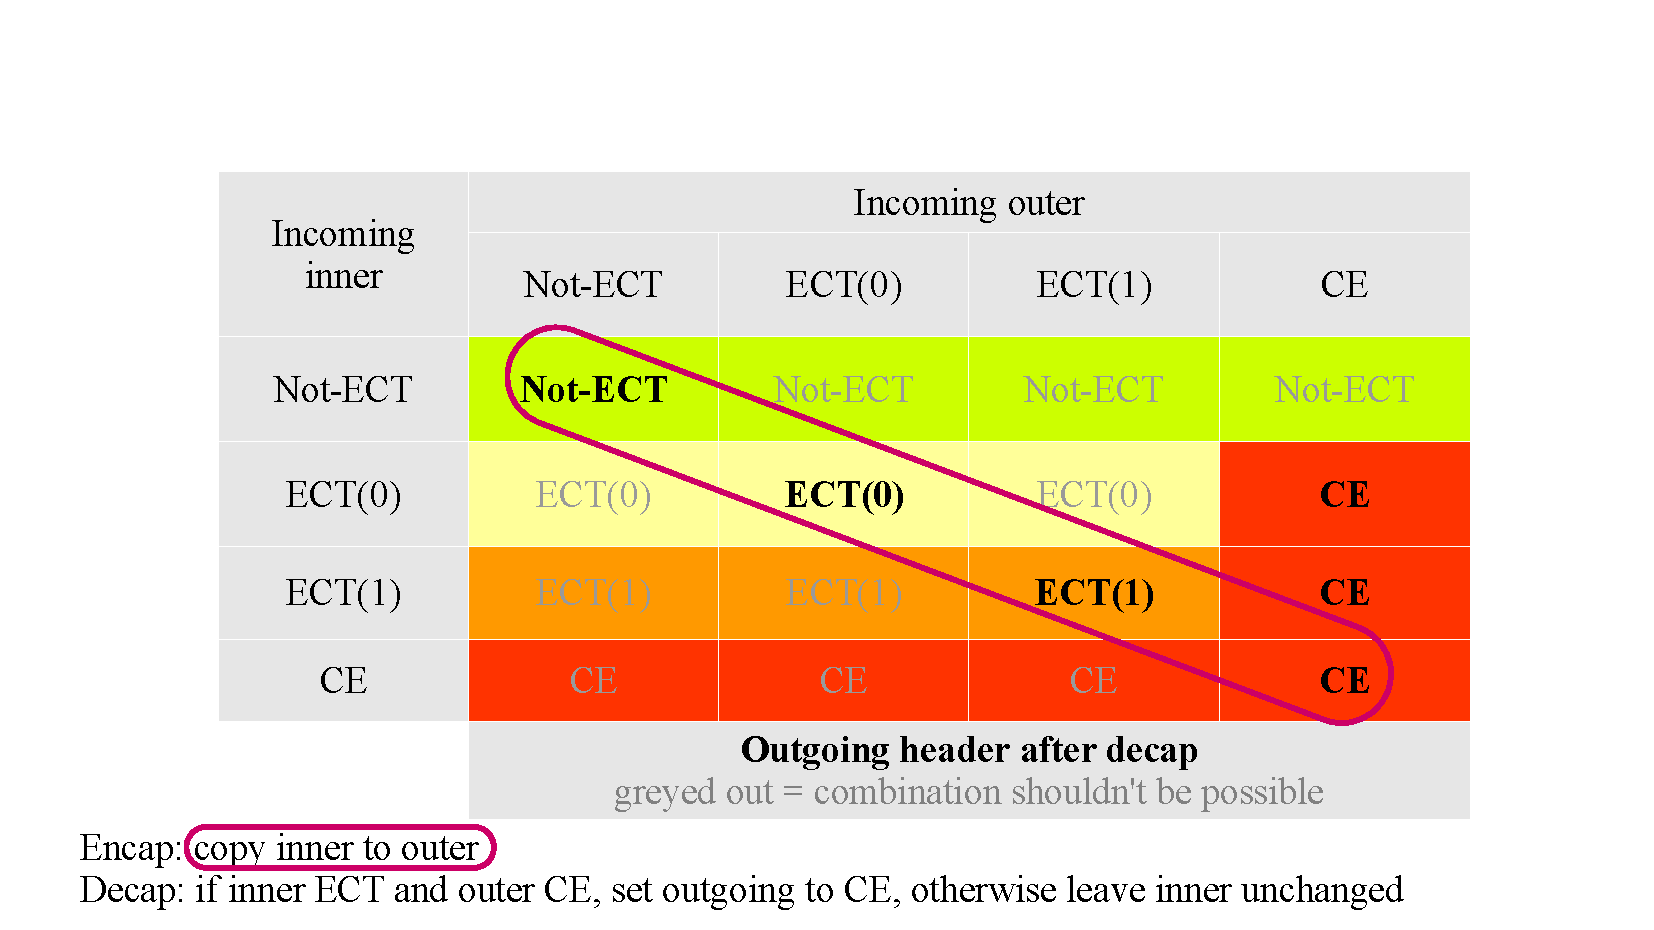
\includegraphics[width=\linewidth,clip]{ecn-tunnel-testing-bg-3}
	\caption{IPsec v2 (RFC~4301)~\cite{IETF_RFC4301:IPSEC_architecture}}\label{fig:ecn-tunnel-testing-bg-3}
\end{figure}
\begin{figure}[h]
	\centering
	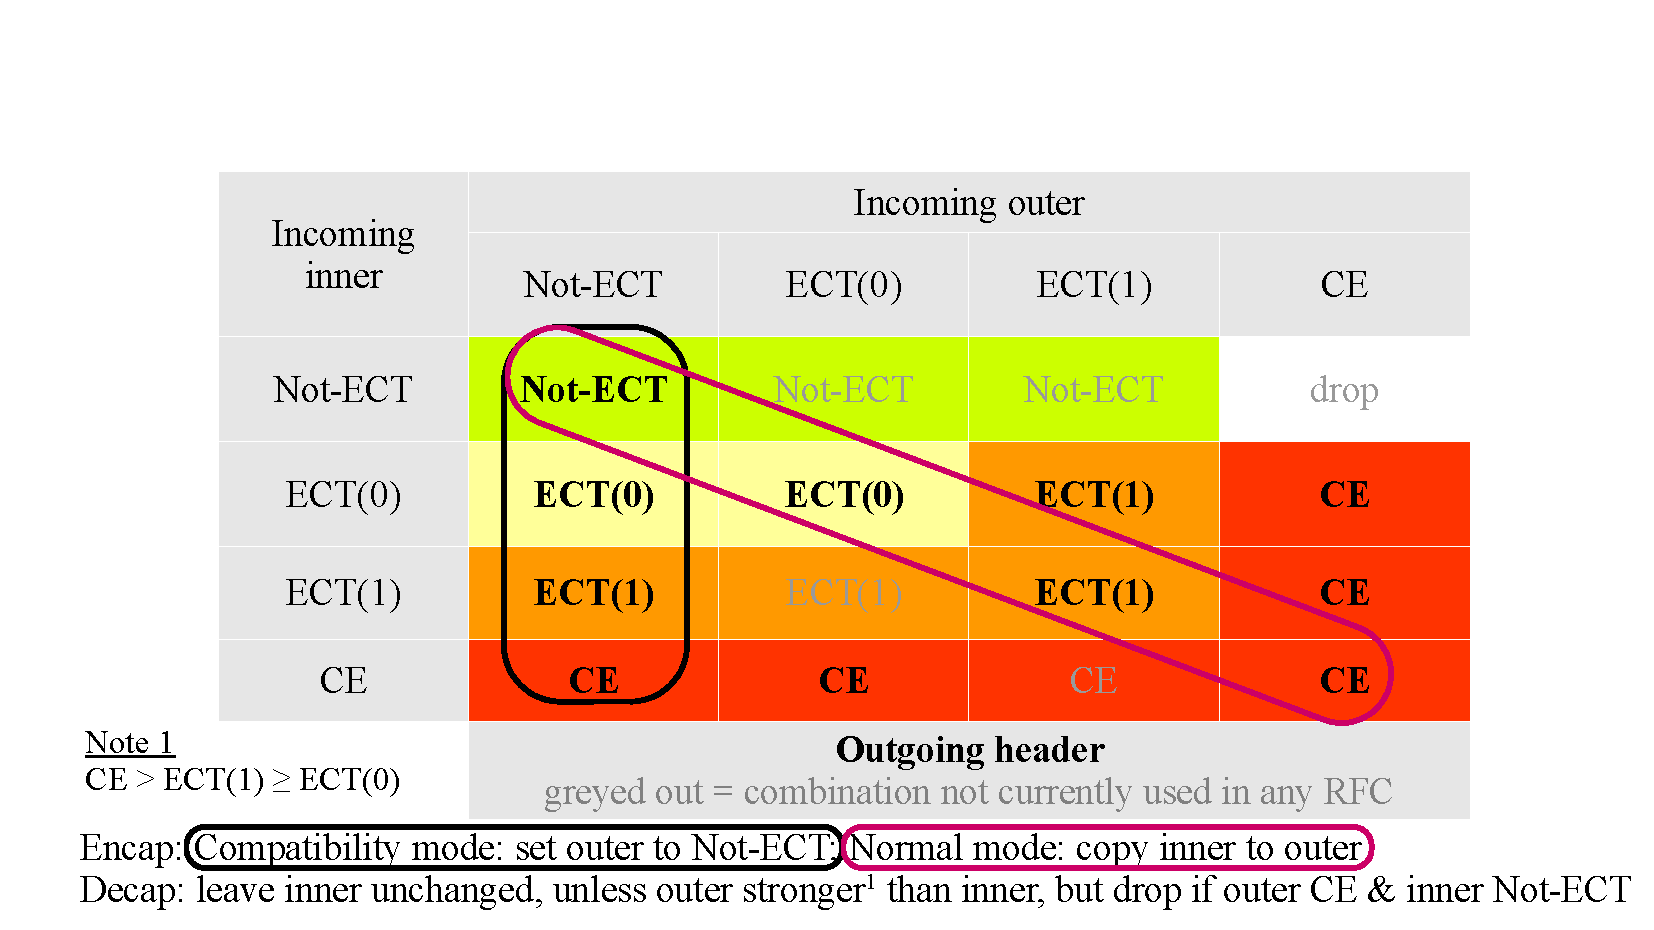
\includegraphics[width=\linewidth,clip]{ecn-tunnel-testing-bg-4}
	\caption{Universal ECN tunnel (RFC~6040)~\cite{Briscoe07b:ECN-tunnel}}\label{fig:ecn-tunnel-testing-bg-4}
\end{figure}

The text in cells outside the loops is greyed out to illustrate that this combination would not be expected. Nonetheless, some other combinations of Inner and Outer can occur when an encap complying with one spec is paired with a decap complying with another. \autoref{fig:ecn-tunnel-testing-bg-5} overlays the three behaviours that correctly propagate ECN to show how the three specs interact with each other. It shows the union of all three possible encap behaviours as not greyed out text, and two colours are used for the cell background where there are two possible decap behaviours.

\begin{figure}[h]
	\centering
	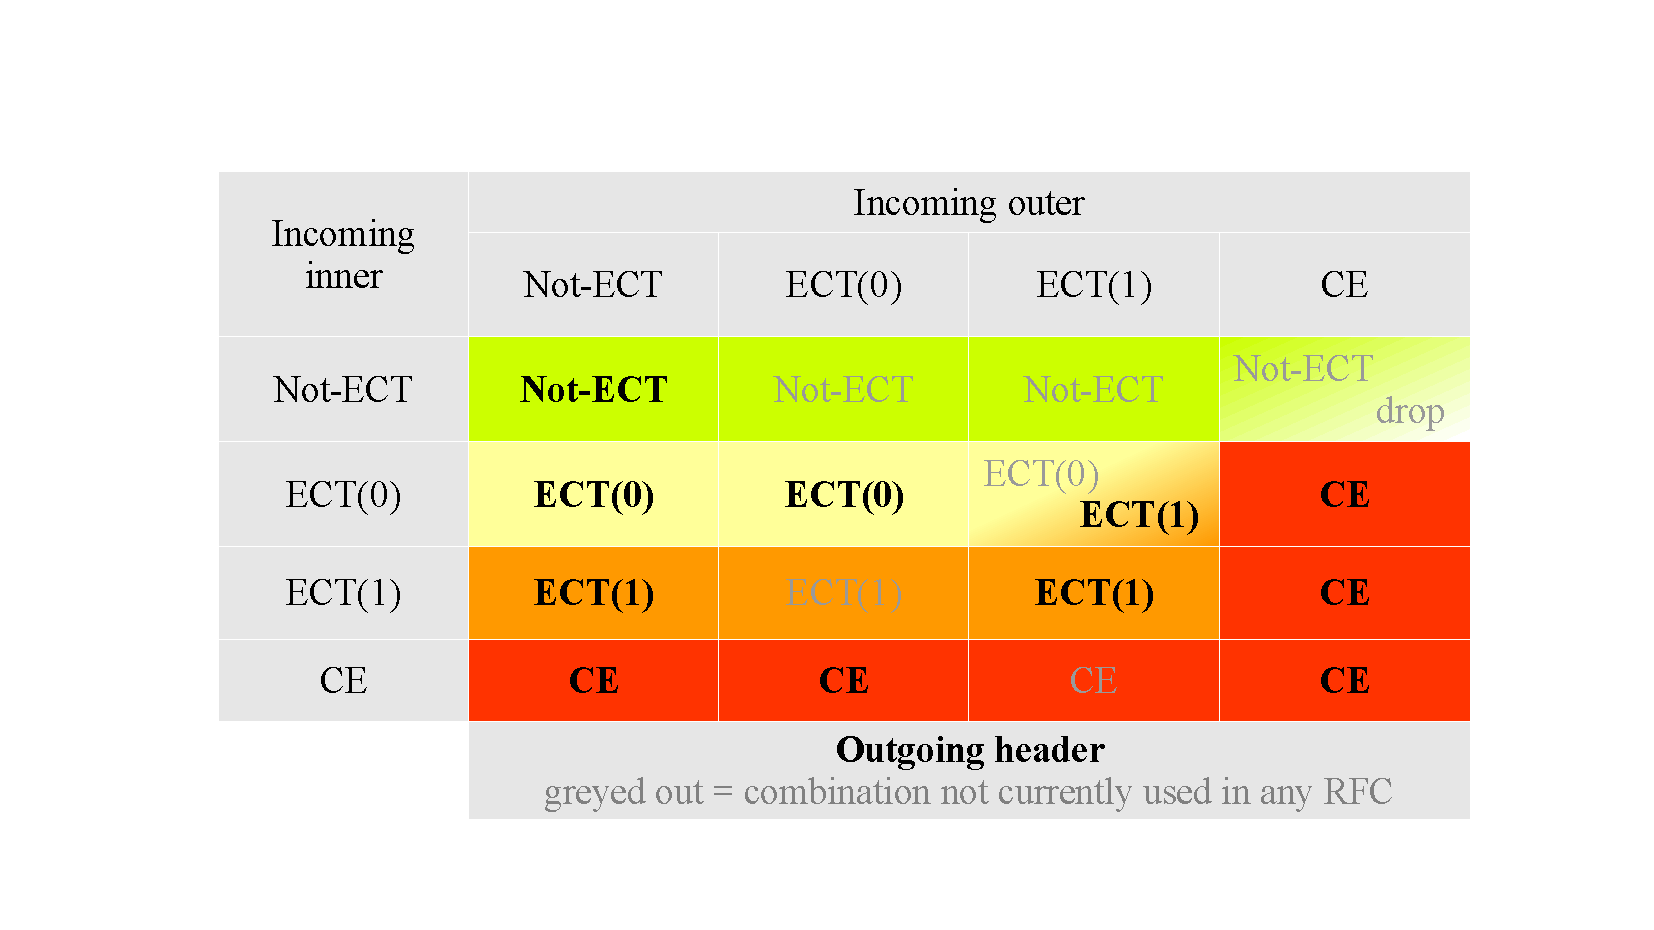
\includegraphics[width=\linewidth,clip]{ecn-tunnel-testing-bg-5}
	\caption{Black box view of all three combinations of ECN-tunnel specs (Figures \ref{fig:ecn-tunnel-testing-bg-2}--\ref{fig:ecn-tunnel-testing-bg-4})}\label{fig:ecn-tunnel-testing-bg-5}
\end{figure}





      % Background
\onecolumn%
% ----------------------------------------------------------------

\onecolumn%
\addcontentsline{toc}{part}{Document history}
\section*{Document history}

\begin{tabular}{|c|c|c|p{3.5in}|}
 \hline
Version &Date &Author &Details of change \\
 \hline\hline
00A          &28 Nov 2023&Bob Briscoe &First Draft\\\hline%
\metaversion &\metadate  &Bob Briscoe &First Issue\\\hline%
\hline%
\end{tabular}

\end{document}

% ----------------------------------------------------------------

%Useful section headers
%% ================================================================
%\section{}\label{ecn-encap-test_}
%
%% ----------------------------------------------------------------
%\subsection{}\label{ecn-encap-test_}
%
%% - - - - - - - - - - - - - - - - - - - - - - - - - - - - - - - -
%\subsubsection{}\label{ecn-encap-test_}
